%%%%%%%%%%%%%%%%%%%%%%%%%%%%%%%%%%%%%%%%%
% Beamer Presentation
% LaTeX Template
% Version 1.0 (10/11/12)
%
% This template has been downloaded from:
% http://www.LaTeXTemplates.com
%
% License:
% CC BY-NC-SA 3.0 (http://creativecommons.org/licenses/by-nc-sa/3.0/)
%
%%%%%%%%%%%%%%%%%%%%%%%%%%%%%%%%%%%%%%%%%

%----------------------------------------------------------------------------------------
%	PACKAGES AND THEMES
%----------------------------------------------------------------------------------------

\documentclass[handout]{beamer}

\mode<presentation> {

% The Beamer class comes with a number of default slide themes
% which change the colors and layouts of slides. Below this is a list
% of all the themes, uncomment each in turn to see what they look like.

%\usetheme{default}
%\usetheme{AnnArbor}
%\usetheme{Antibes}
%\usetheme{Bergen}
%\usetheme{Berkeley}
%\usetheme{Berlin}
%\usetheme{Boadilla}
%\usetheme{CambridgeUS}
%\usetheme{Copenhagen}
%\usetheme{Darmstadt}
%\usetheme{Dresden}
%\usetheme{Frankfurt}
%\usetheme{Goettingen}
%\usetheme{Hannover}
%\usetheme{Ilmenau}
%\usetheme{JuanLesPins}
%\usetheme{Luebeck}
\usetheme{Madrid}
%\usetheme{Malmoe}
%\usetheme{Marburg}
%\usetheme{Montpellier}
%\usetheme{PaloAlto}
%\usetheme{Pittsburgh}
%\usetheme{Rochester}
%\usetheme{Singapore}
%\usetheme{Szeged}
%\usetheme{Warsaw}

% As well as themes, the Beamer class has a number of color themes
% for any slide theme. Uncomment each of these in turn to see how it
% changes the colors of your current slide theme.

%\usecolortheme{albatross}
%\usecolortheme{beaver}
%\usecolortheme{beetle}
%\usecolortheme{crane}
%\usecolortheme{dolphin}
%\usecolortheme{dove}
%\usecolortheme{fly}
%\usecolortheme{lily}
%\usecolortheme{orchid}
%\usecolortheme{rose}
%\usecolortheme{seagull}
%\usecolortheme{seahorse}
%\usecolortheme{whale}
%\usecolortheme{wolverine}

%\setbeamertemplate{footline} % To remove the footer line in all slides uncomment this line
%\setbeamertemplate{footline}[page number] % To replace the footer line in all slides with a simple slide count uncomment this line

%\setbeamertemplate{navigation symbols}{} % To remove the navigation symbols from the bottom of all slides uncomment this line
}

\usepackage{graphicx} % Allows including images
\usepackage{booktabs} % Allows the use of \toprule, \midrule and \bottomrule in tables
\usepackage{cool}
\usepackage{tikz}
\usepackage{amsmath}
\usepackage{xcolor}
\usepackage{hyperref}
\usepackage{bm}

\DeclareMathOperator*{\argmax}{argmax}
\DeclareMathOperator*{\argmin}{argmin}
\usetikzlibrary{positioning}

%----------------------------------------------------------------------------------------
%	TITLE PAGE
%----------------------------------------------------------------------------------------

\title[RL for Finance and Retail]{RL in Finance and Retail Industries} % The short title appears at the bottom of every slide, the full title is only on the title page

\author{Ashwin Rao} % Your name
\institute[Stanford] % Your institution as it will appear on the bottom of every slide, may be shorthand to save space
{Stanford University
 % Your institution for the title page
}

\date{} % Date, can be changed to a custom date

\begin{document}
\begin{frame}
\titlepage % Print the title page as the first slide
\end{frame}

% \begin{frame}
% \frametitle{Overview} % Table of contents slide, comment this block out to remove it
% \tableofcontents % Throughout your presentation, if you choose to use \section{} and \subsection{} commands, these will automatically be printed on this slide as an overview of your presentation
% \end{frame}

\begin{frame}
\frametitle{Machine Learning Types}
\begin{center}
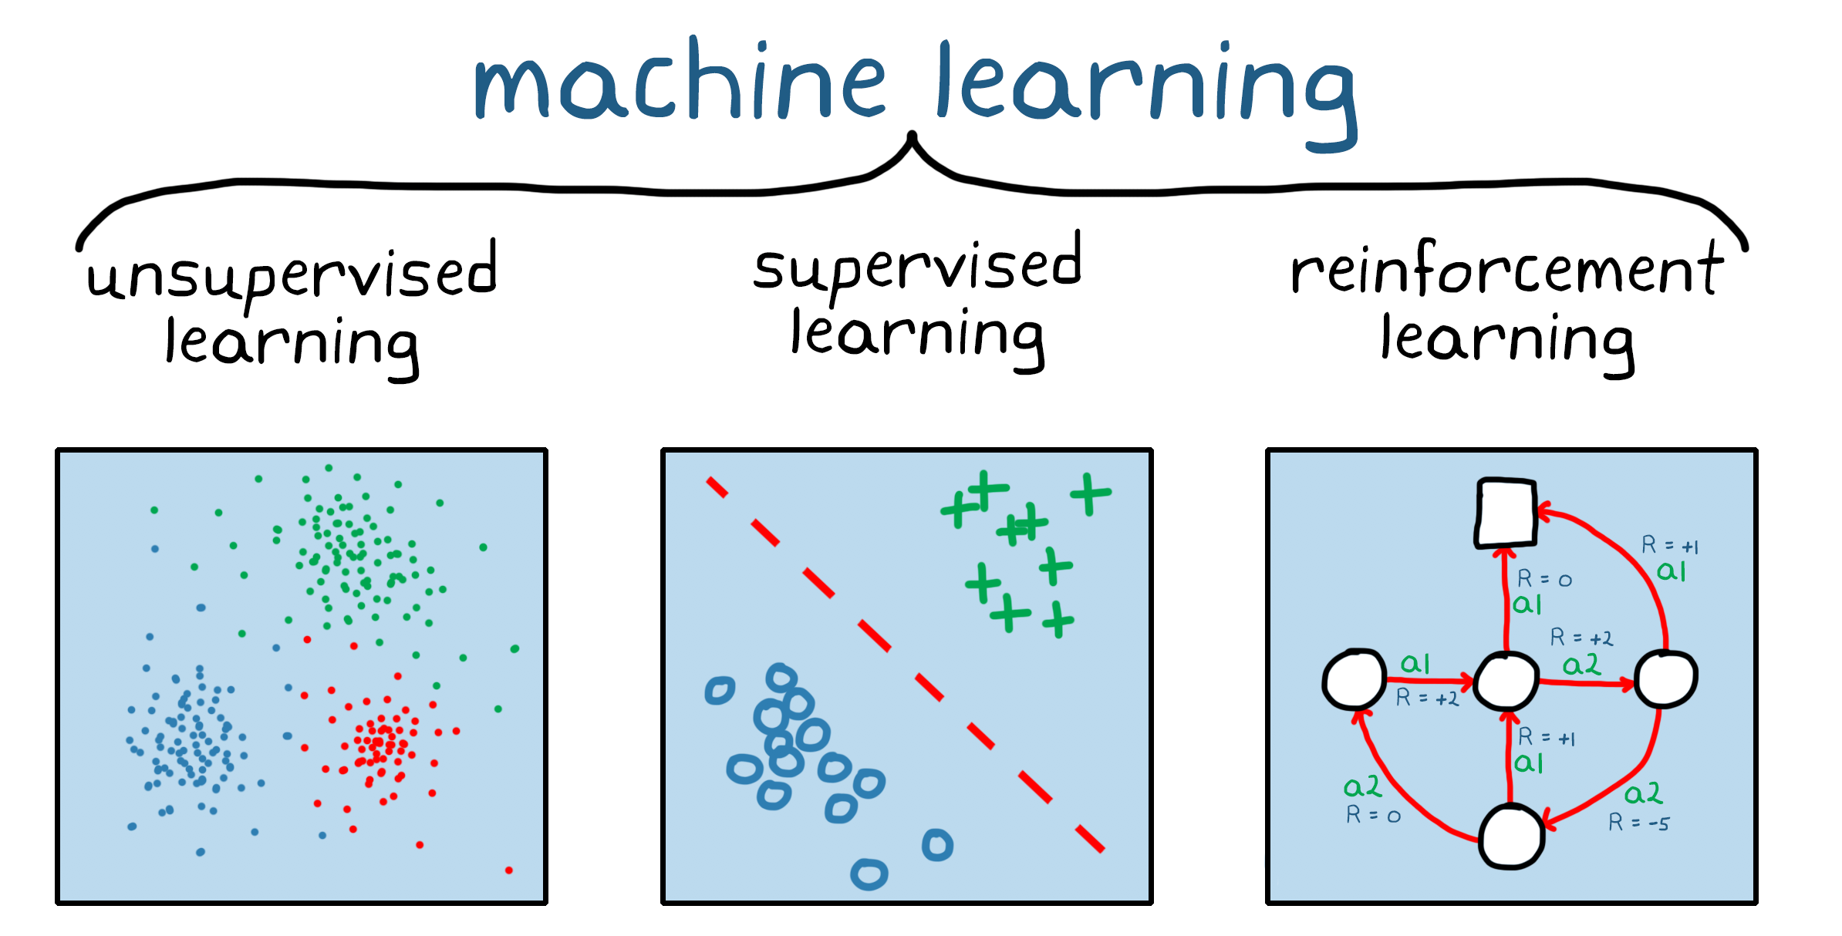
\includegraphics[width=12cm, height=7cm]{ml_types.png}
\end{center}
\end{frame}


\begin{frame}
\frametitle{RL Process - {\em Actions} maximizing {\em Returns} in each {\em State}}
\begin{center}
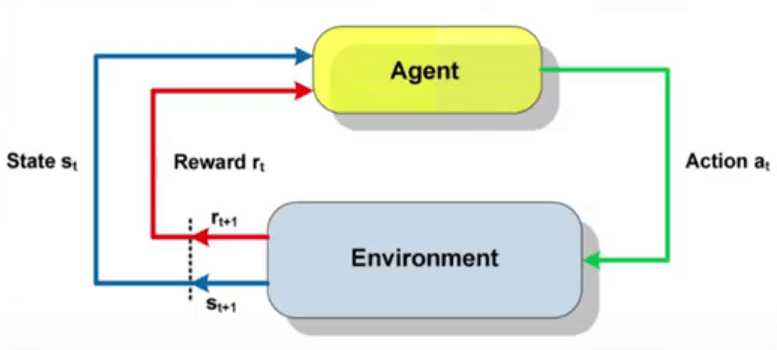
\includegraphics[width=12cm, height=7cm]{RL_diagram.jpg}
\end{center}
\end{frame}


\begin{frame}
\frametitle{Many real-world problems fit this framework}
\pause
\begin{itemize}[<+->]
\item Self-driving vehicle (speed/steering to optimize safety/time)
\item Game of Chess (Boolean {\em Reward} at end of game)
\item Complex Logistical Operations (eg: movements in a Warehouse)
\item Make a humanoid robot walk/run on difficult terrains
\item Manage an investment portfolio
\item Control a power station
\item Optimal decisions during a football game
\item Strategy to win an election (highly complex)
\end{itemize}
\end{frame}


\begin{frame}
\frametitle{Richard Bellman's Equation (from 75 years ago)}
\pause
$$V^*(s) = \max_a  \sum_{s'} \mathcal{P}(s,a,s') \cdot (\mathcal{R}(s,a,s') + \gamma \cdot V^*(s'))$$
\begin{itemize}[<+->]
\item Recursive formulation of the Optimal Expected Return
\item Gave us elegant Dynamic Programming algorithms
\item Assuming we have a model of transition probabilities
\item Impractical, doesn't scale (Curse of Dimensionality/Modeling)
\item To resolve both curses effectively, we need RL
\end{itemize}
\end{frame}

\begin{frame}
\frametitle{Reinforcement Learning (RL)}
\pause
\begin{itemize}[<+->]

\item RL is a ``trial-and-error'' approach linking {\em Actions} to {\em Returns}
\item Try different actions \& learn what works, what doesn't
\item RL incrementally learns from a stream of data through interactions
\item Typically interacting with a {\em simulated} environment ({\em sampling model})
\item {\bf Core Sauce}: Sampling \& Function Approximation come together
\item Deep Neural Networks for function approx. was RL's game-changer
\end{itemize}
\end{frame}

\begin{frame}
\frametitle{Future of RL}
\pause
\begin{itemize}[<+->]

\item {\bf Promise of modern A.I. is based on success of RL algorithms}
\item Agents that efficiently adapt to changing circumstances
\item Sequentially optimizing to achieve business goals
\item Possibilities in Finance and Retail industries are endless 
\end{itemize}
\end{frame}


\begin{frame}
\frametitle{Dynamic Asset-Allocation and Consumption}
\pause
\begin{itemize}[<+->]
\item The broad topic is Investment Management
\item Applies to Corporations as well as Individuals
\item The two considerations are:
\pause
\begin{itemize}[<+->]
\item How to allocate money across assets in one's investment portfolio
\item How much to consume for one's needs/operations/pleasures
\end{itemize}
\item Asset-Allocation and Consumption decisions at each time step
\item Asset-Allocation decisions typically deal with Risk-Reward tradeoffs
\item Consumption decisions are about spending now or later
\end{itemize}
\end{frame}

\begin{frame}
\frametitle{Consider the simple example of Personal Finance}
\pause
\begin{itemize}[<+->]
\item Broadly speaking, Personal Finance involves the following aspects:
\pause
\begin{itemize}[<+->]
\item Receiving Money: Salary, Bonus, Rental income, Asset Liquidation etc.
\item Consuming Money: Food, Clothes, Rent/Mortgage, Car, Vacations etc.
\item Investing Money: Savings account, Stocks, Real-estate, Gold etc.
\end{itemize}
\item Goal: Maximize lifetime-aggregated Expected Utility of Consumption
\item We can model this in the RL framework as follows:
\item {\em State:} Age, Asset Holdings, Asset Valuation, Career situation etc.
\item {\em Action:} Changes in Asset Holdings, Optional Consumption
\item {\em Reward:} Utility of Consumption of Money
\item {\em Model:} Career uncertainties, Asset market uncertainties
\end{itemize}
\end{frame}


\begin{frame}
\frametitle{Trading Order Book - various applications of RL}
\includegraphics[width=11.5cm, height=7cm]{cme241/order_book.png}
\end{frame}

\begin{frame}
\frametitle{Some more applications I've been excited about}
\begin{itemize}[<+->]
\item Financial Derivatives Pricing and Hedging
\item Inventory Control in Supply-Chain
\item Promotional Pricing and Clearance Pricing
\end{itemize}
\end{frame}


\begin{frame}
\frametitle{Book}
\begin{center}

\includegraphics[width=5.5cm, height=8cm]{RLBook.jpeg}
\end{center}
\end{frame}


\end{document}